\vspace{1cm}
\newline
\lecture{4}{14/10/2021}
\vspace{0.5cm}
\section{Sfera di Bloch}
Esiste un modo di rappresentare lo stato di un qubit, in maniera grafica, attraverso l'utilizzo della \textbf{sfera di Bloch}. Questo espediente è comodo per comprendere che cosa sta avvenendo allo stato di un qubit, lo svantaggio principale riguarda la sua applicabilità, in quanto è possibile usarlo per singoli qubit. Come al solito noi utilizziamo la matrice densità $\hat \rho$ piuttosto che la funzione d'onda $\psi$ per descrivere lo stato di un sistema a due livelli\footnote{Nel caso di un qubit, la matrice densità è rappresentata da una matrice $2\times2$}:
\begin{equation*}
    \hat \rho = \begin{pmatrix}
                    \rho_{00} & \rho_{01} \\
                    \rho_{10} & \rho_{11}
                \end{pmatrix} \, ,
\end{equation*}
dove $\rho_{00}$, $\rho_{11} \in \mathbb{R}$, $\rho_{11}=1-\rho_{00}$ e $\rho_{01}=\rho_{10}^*$. A questo punto ridefiniamo gli elementi di $\hat \rho$ come
\begin{equation*}
    \rho_{00}=\alpha \quad \, , \quad \rho_{11}=1-\alpha \quad \, , \quad \rho_{01}=\beta + i\gamma \quad \, , \quad \rho_{10}=\beta - i \gamma
\end{equation*}
dove $\alpha, \beta$ e $\gamma \in \mathbb{R}$. \\
Se consideriamo l'insieme di matrici dato dall'identità e dalle matrici di Pauli $\{\mathbb{I}, \sigma_1, \sigma_2, \sigma_3 \}$ possiamo riscrivere la matrice densità in una forma particolarmente interessante
\begin{equation*}
    \hat \rho = a\mathbb{I} + \sum_{i=1}^3 c_i\sigma_i \, ,
\end{equation*}
siccome $\Tr(\hat \rho)\overset{!}{=}1$, allora dal momento che $\Tr(\sigma_i)=0$ e $\Tr(\mathbb{I})=2$ abbiamo che $a=\frac 12$.
\begin{equation*}
    \hat \rho = \frac 12\left(\mathbb{I}+\sum_{i=1}^3 p_i \sigma_i\right) \, .
\end{equation*}
Cosa sono i $p_i$? Osserviamo che $\Tr(\hat \rho \sigma_i)=p_i=\expval{\sigma_i}$, cioè corrispondono ai valori di aspettazione della corrispondente matrice di Pauli tracciata insieme alla matrice densità.\\
A questo punto possiamo prendere i $p_i$ come le componenti di un vettore $\vec{p}=(p_1, p_2, p_3)$ che si trova all'interno della sfera di Bloch come possiamo vedere in Figura \ref{fig:BlochSphere}.
In particolare notiamo che
\begin{itemize}
    \item Se $\hat \rho$ è \textbf{puro}, $\hat \rho=\op{\psi}{\psi}$, dove
    \begin{equation*}
        \ket \psi = \cos \frac \theta 2 \ket 0 + e^{i\phi}\sin \frac \theta 2 \ket 1
    \end{equation*}
    $\hat \rho$ e $\psi$ rappresentano lo stesso stato sulla sfera di Bloch, è situato sulla superficie della sfera;
    \item Se $\hat \rho$ è una \textbf{miscela}
    \begin{equation*}
        \hat \rho = \begin{pmatrix}
                        \frac{1+p_z}{2} & \frac{p_x-ip_y}{2} \\
                        \frac{p_x+ip_y}{2} & \frac{1-p_z}{2}
                    \end{pmatrix}
    \end{equation*}
    e calcolassimo $\rho^2$ e poi $\Tr(\rho^2)$ troveremo che
    \begin{equation*}
        \rho^2 = \frac 14 \left(\mathbb{I}+\sum_ip_i \sigma_i + \sum_j p_j \sigma_j + \sum_{ij}p_ip_j\sigma_i\sigma_j\right)
    \end{equation*}
    \begin{equation*}
        \Tr(\rho^2) = \frac 12 + \frac 24 \sum_i p_i^2=\frac 12 \left(1+ \abs{\vec p}^2\right)
    \end{equation*}
    Se $\abs{\vec p}^2$ è minore di 1 allora abbiamo una miscela, la sfera che si ottiene da $\vec p$ è una sfera all'interno di quella unitaria (stato puro).
\end{itemize}
\begin{figure}[!ht]
    \centering
    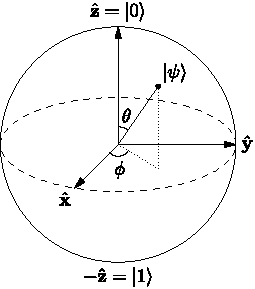
\includegraphics[scale=1.4]{images/Bloch_Sphere.pdf}
    \caption{Rappresentazione generale di un qubit sulla sfera di Bloch.}
    \label{fig:BlochSphere}
\end{figure}
\subsection{Matrice densità termica}
Supponiamo di avere $\hat \rho=\sum_n \omega_n \op{\psi_n}{\psi_n}$, in principio abbiamo molti modi per descrivere il nostro stato da $\ket{\psi_n}$ ognuno con probabilità $\omega_n$. Se il nostro sistema è libero di scambiare energia con l'ambiente abbiamo a che fare con un \textbf{sistema aperto}. Dopo un lungo periodo di tempo di interazione, il nostro sistema raggiungerà un equilibrio, cosicché la nostra probabilità per lo stato $\ket{\psi_n}$ sarà
\begin{equation*}
    \omega_n \equiv \frac{e^{-E_n/k_BT}}{Z} \, ,
\end{equation*}
dove $E_n$ è l'energia dello stato $\ket{\psi_n}$ e $Z=\sum_i e^{-E_i/k_BT}$ è la funzione di partizione canonica.\\
Se prendiamo la base $\ket n$ tale per cui $\hat H \ket n = E_n \ket n$ abbiamo
\begin{equation*}
    \hat \rho = \frac{e^{-\hat H/k_BT}}{Z}\, , \qquad Z=\Tr(e^{-\hat H/k_BT})=1\, , \qquad \rho_{mn}=\mel{m}{\hat \rho}{n}=\frac{e^{-E_n/k_BT}}{Z}\delta_{mn}\equiv \omega_n\, .
\end{equation*}
Usando la base computazionale $\{\ket 0, \ket 1\}$, con energie rispettivamente $E_0$, $E_1$, la matrice densità sarà
\begin{align*}
    \rho &= a_0 \op{0}{0} + a_1 \op{1}{1} \\
         &= \frac{e^{-E_0/k_BT}}{Z}\op{0}{0}+\frac{e^{-E_1/k_BT}}{Z}\op{1}{1}\, ,
\end{align*}
il rapporto tra i due coefficienti è pari a $a_1/a_0=e^{-\Delta E/k_BT}$ quindi possiamo osservare che se
\begin{itemize}
    \item $k_BT \gg \Delta E$, $a_1/a_0 \rightarrow 1$ la matrice densità è una miscela. Il sistema sarà portato allo stato massimamente miscelato (al centro della sfera di Bloch).
    \item $k_BT \ll \Delta E$, $a_1/a_0 \rightarrow 0$, $a_0 \rightarrow 1$ la matrice densità è uno stato puro, poiché il sistema disperde la sua energia nell'ambiente e decade nel suo stato fondamentale.
\end{itemize}
\section{Sistemi compositi}
Utilizziamo sistemi quantistici per studiarne i comportamenti quantistici, per farlo dobbiamo interagire con questi oggetti per misurare qualche loro proprietà, ad esempio sistemi macroscopici, come i rivelatori, interagiscono con sistemi microscopici. Dobbiamo trovare le connessioni che vi sono tra rivelatore e sistema. La terza componente che subentra tra rivelatore e sistema quantistico è l'ambiente, a differenza degli altri due, la sua trattazione è molto complessa per cui rimuoviamo l'ambiente e trattiamo il sistema composito rivelatore e sistema. \\
Trovando un modo di rimuovere l'ambiente dal nostro sistema composito, consideriamo due sistemi descritti rispettivamente da due spazi di Hilbert $\mathcal{H}_1$ e $\mathcal{H}_2$. Il sistema composito è dato da $\mathcal{H}_1\otimes\mathcal{H}_2=\mathcal{H}$. Se $\text{dim}\mathcal{H}_1 = n$ e $\text{dim}\mathcal{H}_2 = m$, allora $\text{dim}\mathcal{H} = n\times m$. Introduciamo l'ultimo postulato della meccanica quantistica
\begin{itemize}
    \item \textbf{V Postulato} (\textbf{Sistemi compositi}): Consideriamo un sistema quantistico composto da 2 sottosistemi $1$ e $2$ con spazi di Hilbert $\mathcal{H}_1$ e $\mathcal{H}_2$ rispettivamente. Lo spazio di Hilbert del sistema totale è dato da\footnote{Il simbolo "$\otimes$" indica il \textbf{prodotto tensoriale} tra spazi.} $\mathcal{H} = \mathcal{H}_1 \otimes \mathcal{H}_2$.
\end{itemize}
Se $\ket{\psi}_1\in\mathcal{H}_1$ e $\ket{\psi}_2\in\mathcal{H}_2$, allora $\ket{\psi}_1\otimes\ket{\psi}_2\in\mathcal{H}$, più precisamente se $\ket{n}_1$ e $\ket{m}_2$ sono una base per $\mathcal{H}_1$ e $\mathcal{H}_2$, allora $\ket{nm}$ è una base per $\mathcal{H}$. \\
Quando $n=m=2$, allora $\ket{nm}=\{\ket{00}, \ket{01}, \ket{10}, \ket{11}\}$ e $\ket \psi \in \mathcal{H}$ è scrivibile come $\ket{\psi}=\sum_{n,m}a_{nm}\ket{nm}$. \\
Introduciamo gli \textbf{stati separabili}, come suggerisce il nome si tratta di stati che possono essere trattati separatamente e si possono combinare le rispettive soluzioni in un secondo momento, infatti
\begin{equation*}
    \underbrace{\ket{\psi_1}}_{= \ket 0, \ket 1}\otimes\underbrace{\ket{\psi_2}}_{= \ket 0, \ket 1}=\alpha a \ket{00} + \alpha b \ket{01} + \beta a \ket{10} + \beta b \ket{11}
\end{equation*}
Accanto agli stati, abbiamo gli operatori che lavorano in questo spazio $\mathcal{H}$, per esempio se $\hat A \in L(\mathcal{H}_1)$, $\hat B \in L(\mathcal{H}_1)$, allora $\hat U = \hat A \otimes \hat B$. Quest'ultimo operatore agisce nel seguente modo
\begin{equation*}
    \hat U \ket \psi = \hat A \otimes \hat B(\ket{\psi_1}\otimes\ket{\psi_2})=\hat A\ket{\psi_1}\otimes \hat B\ket{\psi_2}
\end{equation*}
Perché ci interessa? Perché questi operatori possono essere associati ad osservabili! Come realizziamo una misura su un sistema composito? Supponiamo di avere
\begin{equation*}
    \tilde{A}=A\otimes \mathbb{I} \Rightarrow \tilde{A}: \mathcal{H} \rightarrow \mathcal{H}
\end{equation*}
$\hat A$ rappresenta la misura su un sistema di qubit mentre $\hat B$ l'identità. In questo caso $\hat A$ possiede due proiettori
\begin{equation*}
    P_A^0 = \op{0}{0} \qquad P_A^1=\op{1}{1} \, ,
\end{equation*}
e vogliamo andare a valutare
\begin{equation*}
    \expval{\tilde{A}}=\expval{A\otimes \mathbb{I}}=\mel{\psi}{A \otimes \mathbb{I}}{\psi}=\sum_{ijk}a_{ij}^*a_{kj}\mel{i}{A}{k} \, ,
\end{equation*}
dove ovviamente $\ket \psi \in \mathcal{H}, \ket \psi = \sum_{ij}a_{ij}\ket{ij}$.\\
Otteniamo così
\begin{equation*}
    \expval{\tilde{A}}=\sum_{ij}a_{ij}^2\mel{i}{A}{j} \, .
\end{equation*}
La funzione d'onda che andiamo a considerare è data da $\ket{\psi_1}\otimes\ket{\psi_2}$ e risulta essere definita come
\begin{equation*}
    \ket \psi = \alpha a \ket{00} + \alpha b \ket{01} + \beta a \ket{10} + \beta b \ket{11}\, ,
\end{equation*}
da cui otteniamo che
\begin{align*}
    &\hat A \ket 0 = \ket 0 \\
    &\hat A \ket 1 = -\ket 1 
\end{align*}
cioè
\begin{equation*}
    \hat A = \begin{pmatrix}1 & 0 \\ 0 & -1 \end{pmatrix}
\end{equation*}
e il suo valore di aspettazione è pari a
\begin{equation*}
    \expval{A}=(\alpha a)^2 + (\alpha b)^2 - (\beta a)^2 - (\beta b)^2 \, .
\end{equation*}
Nel caso in cui
\begin{align*}
    &A\otimes\mathbb{I}\left[\frac{\ket{00}+\ket{01}}{\sqrt 2}\right] \Rightarrow \ket{00}, \ket{01} \quad \text{sono stati separabili} \\
    &A\otimes\mathbb{I}\left[\frac{\ket{01}-\ket{10}}{\sqrt 2}\right] \Rightarrow \ket{01}, \ket{10} \quad \text{sono stati entangled} \\
\end{align*}
\subsection{Matrice densità ridotta}
Se abbiamo uno spazio di Hilbert $\mathcal{H}_A$ e misuriamo l'osservabile $\hat A$ ($a_k$, $\ket{a_k}$, abbiamo una probabilità di ottenere il risultato $a_k$ pari a
\begin{equation*}
    p(a_k)=\Tr\left(\op{a_k}{a_k}\rho\right)=\Tr\left(P_{a_k}\rho\right) \, .
\end{equation*}
Altre informazioni che possiamo ottenere sono
\begin{equation*}
    \expval{A}=\Tr(A\rho) \, ,
\end{equation*}
dove
\begin{equation*}
    \rho \rightarrow \frac{P_{a_k}\rho P_{a_k}}{\sqrt{\Tr{P_{a_k}\rho}}} \, ,
\end{equation*}
questo discorso è valido per un qubit. Supponiamo di considerare ora un qubit connesso a un rivelatore, ambiente, \dots In questo caso lo spazio di Hilbert è dato da $\mathcal{H}_A \otimes \mathcal{H}_B$, in questo caso la matrice densità $\rho^{AB}$ è un operatore appartenere a questo spazio. Vogliamo sapere se possiamo ottenere informazioni sul sottospazio $\mathcal{H}_A$, ignorando completamente $\mathcal{H}_B$, la risposta è affermativa e lo si fa nel seguente modo
\begin{equation*}
    \rho^A = \Tr_B(\rho^{AB}) \, ,
\end{equation*}
questa quantità prende il nome di \textbf{matrice densità ridotta}. Cerchiamo di formalizzare meglio questo risultato. \\
Siano $A:\mathcal{H}_A \rightarrow \mathcal{H}_A$ e $B:\mathcal{H}_B \rightarrow \mathcal{H}_B$ due operatori. La loro combinazione è definita come $A \otimes B:\mathcal{H}_A\otimes \mathcal{H}_B \rightarrow \mathcal{H}_A\otimes\mathcal{H}_B$, la \textbf{traccia parziale} è data da
\begin{align*}
    &\Tr_A : L(\mathcal{H}_A\otimes \mathcal{H}_B) \rightarrow L(\mathcal{H_B}) \\
    &\Tr_B : L(\mathcal{H}_A\otimes \mathcal{H}_B) \rightarrow L(\mathcal{H_A}) \, .
\end{align*}
Consideriamo il seguente esempio
\begin{esempio}
Sia $\rho^{AB}=\rho \otimes \sigma$, vogliamo valutare la traccia parziale sul sottospazio $\mathcal{B}$, in questo caso
\begin{equation*}
    \rho^A = \Tr_B(\rho^{AB})=\Tr_B(\rho \otimes \sigma)=\Tr(\sigma)\rho = \rho
\end{equation*}
questo per quanto riguarda \textbf{stati separabili}, ma in generale non è sempre vero! Infatti supponiamo di considerare
\begin{equation*}
    \rho = \frac{\ket{00}+\ket{11}}{\sqrt 2}\frac{\bra{00}+\bra{11}}{\sqrt 2}
\end{equation*}
se eseguissimo la traccia parziale sul sottospazio $\mathcal{H}_2$, avremmo che
\begin{equation*}
    \rho_1 = \Tr_2\rho = \frac{\mathbb{I}}{2}
\end{equation*}
In questo caso, abbiamo sì che $\Tr (\rho_1)=1$, ma $\Tr(\rho_1^2)=\frac 12$, cioè $\rho_1$ è una miscela di stati!
\end{esempio}